Figures \ref{fig:instersection_purely_relational_floris} and \ref{fig:instersection_purely_relational_pauli} visualize an example application of purely relational factorization. Figure \ref{fig:instersection_purely_relational_floris} shows the intersection of latent topics depicted in Figure \ref{figure:purely_relational_decomposition} with publication data of Floris Geerts, while Figure \ref{fig:instersection_purely_relational_pauli} shows the intersection of the same latent topics with the publication data of Pauli Miettinen. 

The figures show that we can relate not only particular data points such as venues and co-authors between scientists, but also common (latent) topics. They are identified and visualized in an interpretable manner. The intersection includes the publication records (indicated in red) of two authors (the other author is indicated in pink, if he/she belongs to co-authors of the original decomposition). If for a latent variable, there are a co-author, a university and a venue that belong to both authors, then the latent topic is labeled (in blue) as common.
\begin{figure}[htb]
  \begin{center}
      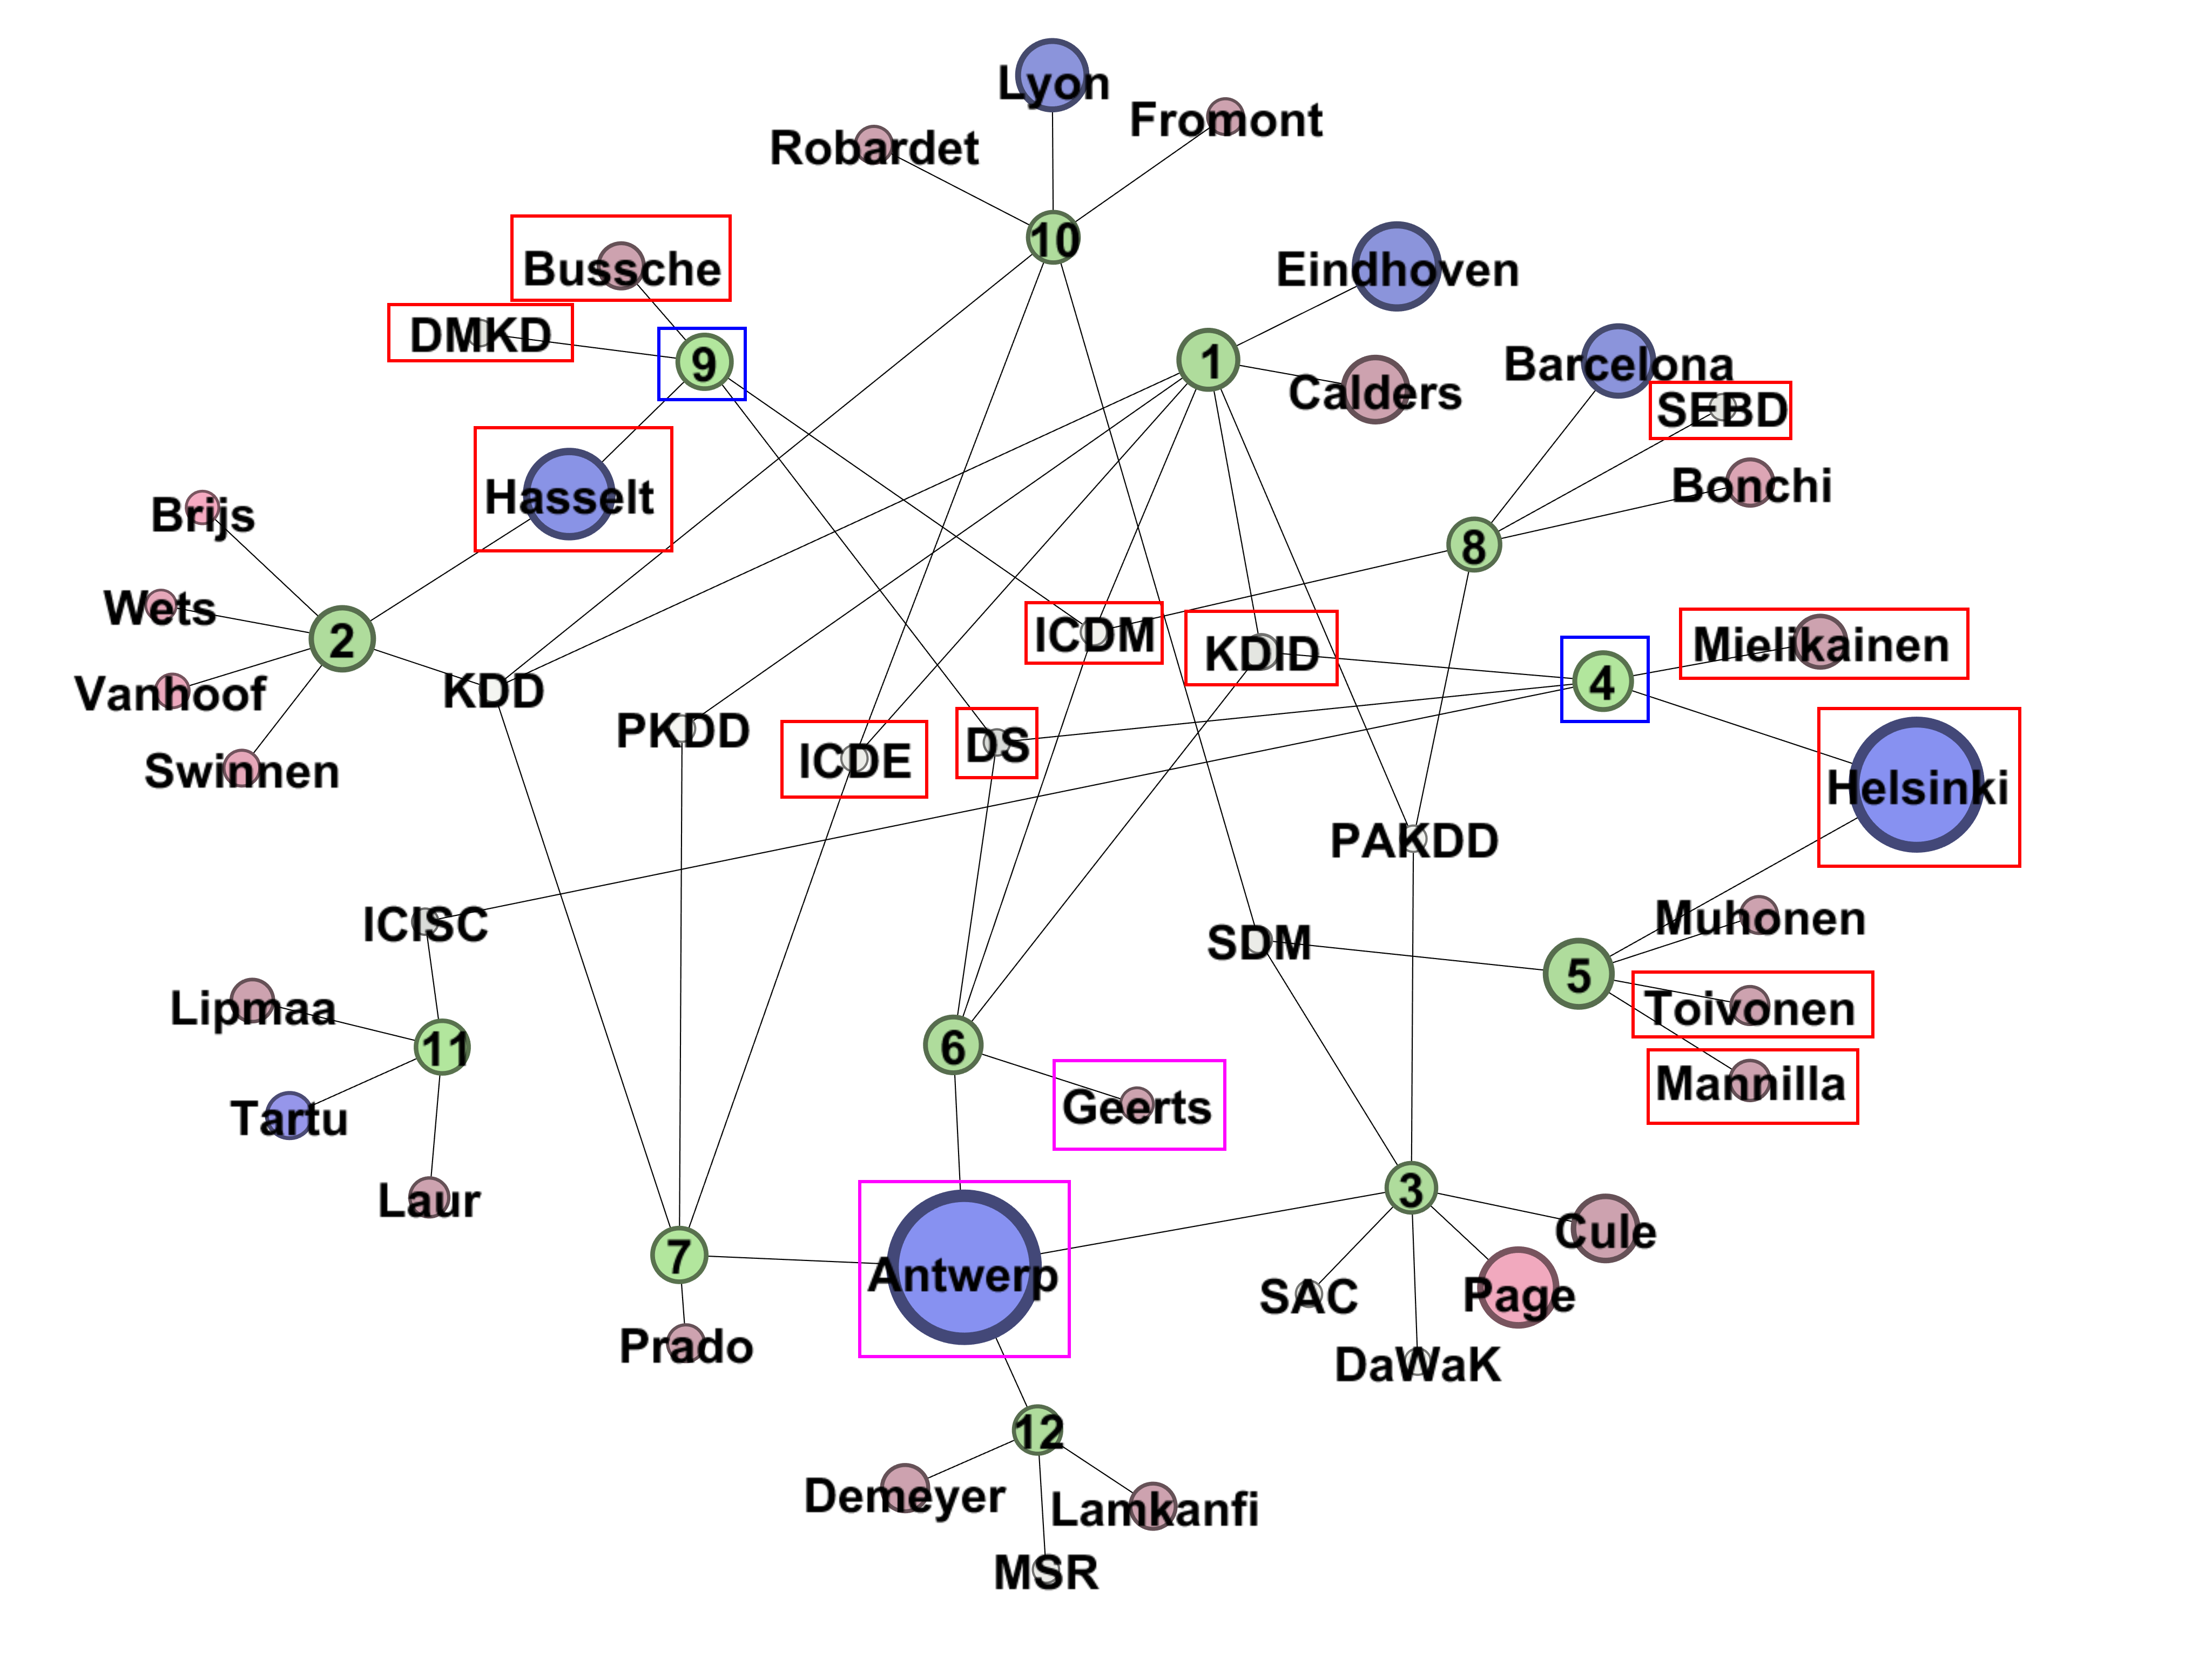
\includegraphics[width=\textwidth]{query_relational_selection_floris_geerts.png}
  \end{center}
  \caption{An application of purely relational factorization: intersection of publication data (in red) and latent topics (in blue) of Bart Goethals with publications of his co-author Floris Geerts (highlighted in pink) in the graph. A latent topic belongs to an intersection if both have the same co-author, university and venue in the publication records.}
  \label{fig:instersection_purely_relational_floris}
\end{figure}

\begin{figure}[htb]
  \begin{center}
      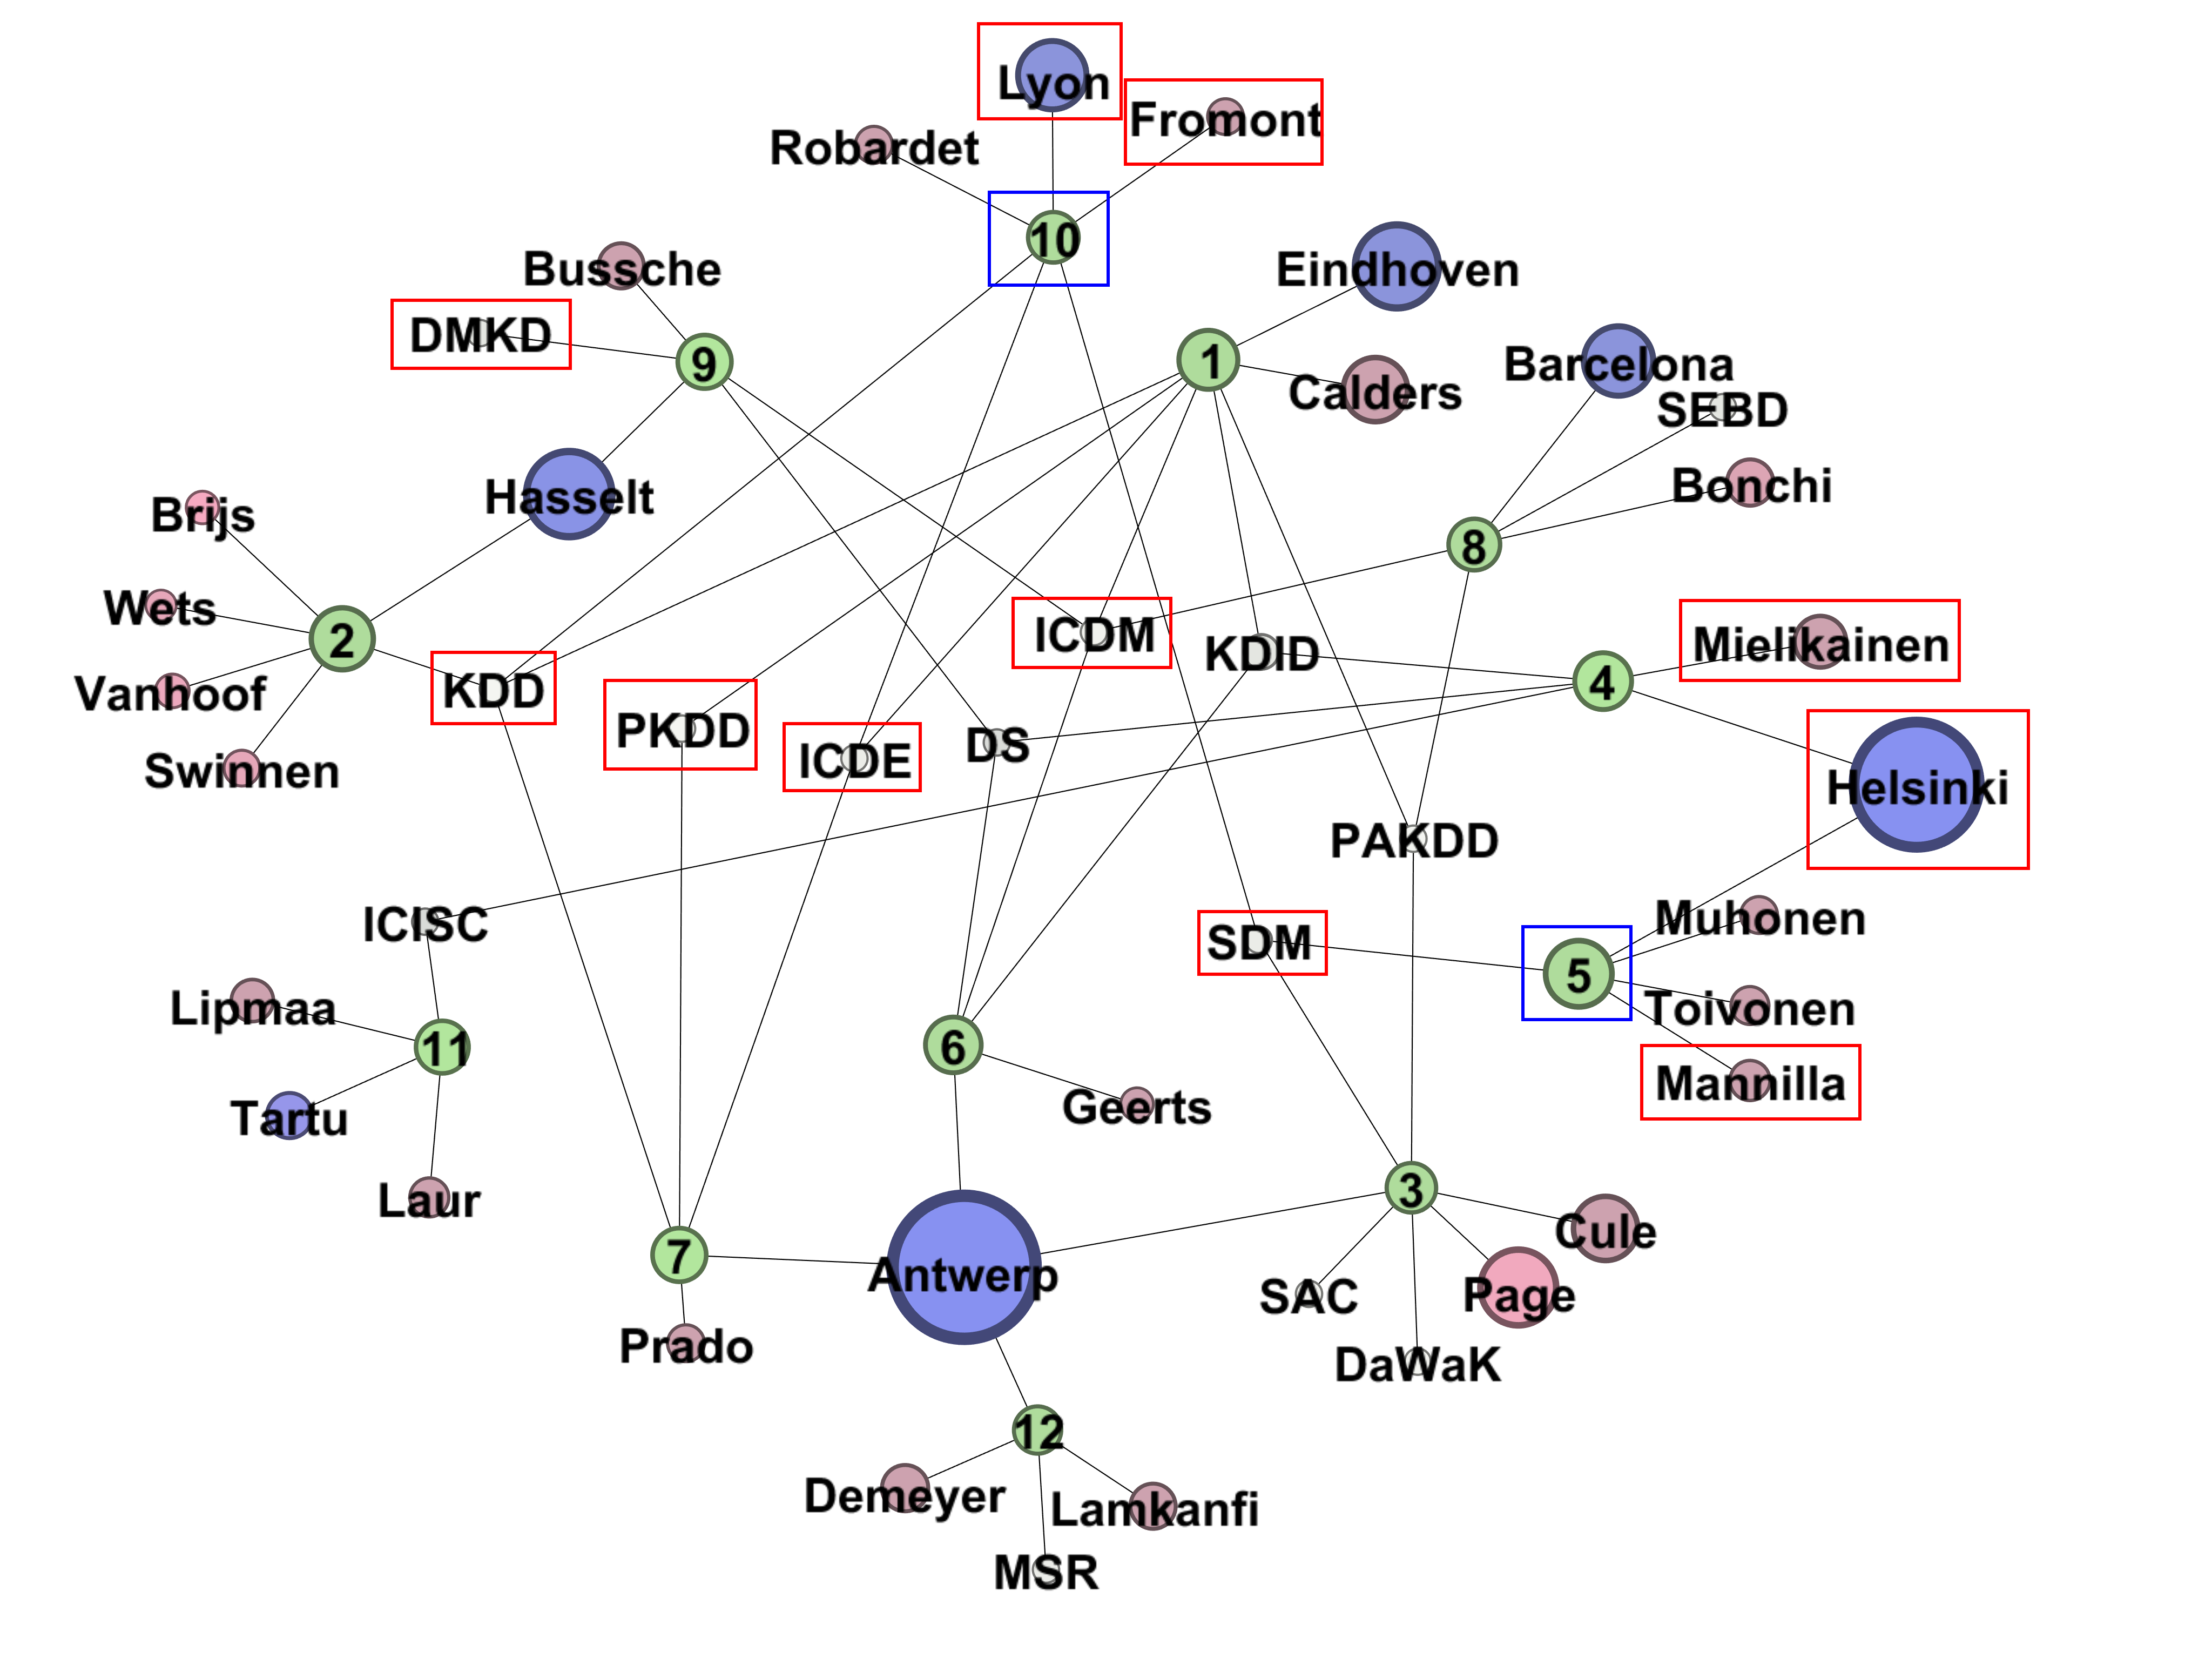
\includegraphics[width=\textwidth]{query_relational_selection_pauli_miettens.png}
  \end{center}
  \caption{An application of purely relational factorization: intersection of publication data (in red) and of latent topics (in blue) of Bart Goethals with publications of Pauli Miettinen (not his co-author). A latent topic belongs to an intersection if both have the same co-author, university and venue in the publication records.}
  \label{fig:instersection_purely_relational_pauli}
\end{figure}


